\section{Исследовательская часть}

\subsection{Исследование на статистических данных за 2020 год}

Реализованный метод исследовался путем проведения моделирования на статистических данных ВУЗов и УГСН за 2020 год и сравнения с результатами приемной кампании того же года. На рисунке \ref{top5tech} представлены результаты для выборки технических ВУЗов. Результаты работы с разбиением по медицинским и гуманитарным категориям представлены на рисунках ниже.

\begin{figure}[hbtp]
	\centering
	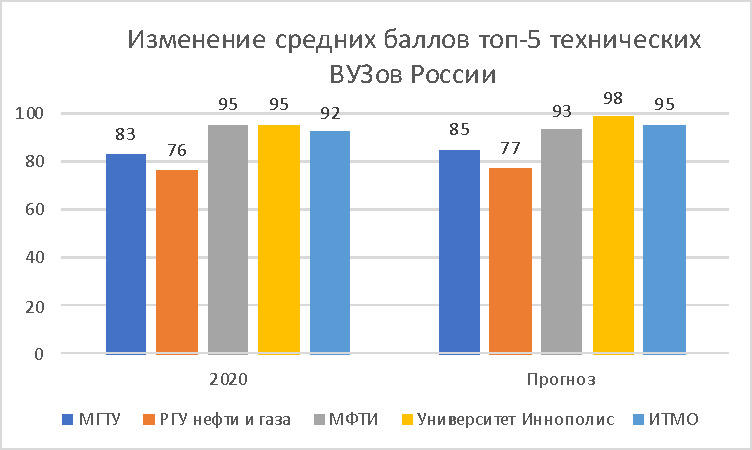
\includegraphics[scale=1.0]{img/top5tech.pdf.pdf}
	\caption{Изменение средних баллов ТОП-5 технических ВУЗов}
	\label{top5tech}
\end{figure} 

\begin{figure}[hbtp]
	\centering
	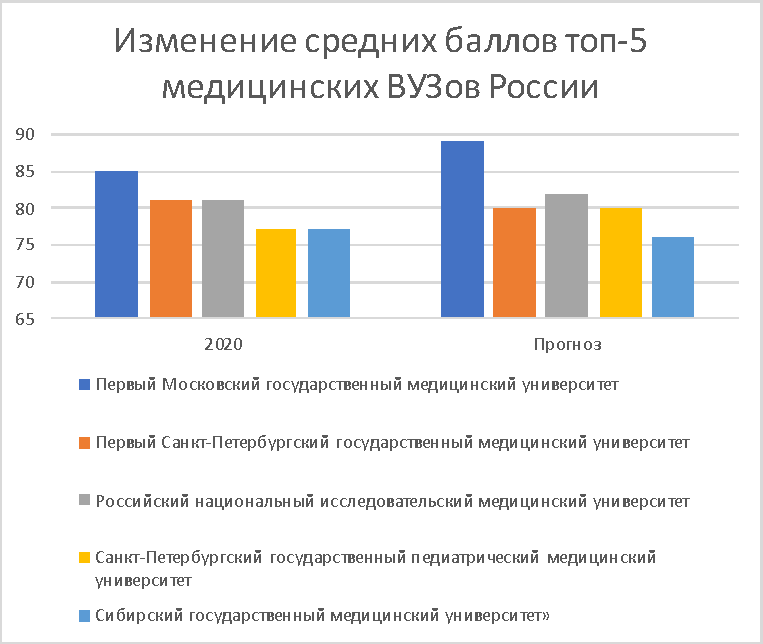
\includegraphics[scale=1.0]{img/top5med.pdf.pdf}
	\caption{Изменение средних баллов ТОП-5 медицинских ВУЗов}
	\label{top5med}
\end{figure} 

\begin{figure}[hbtp]
	\centering
	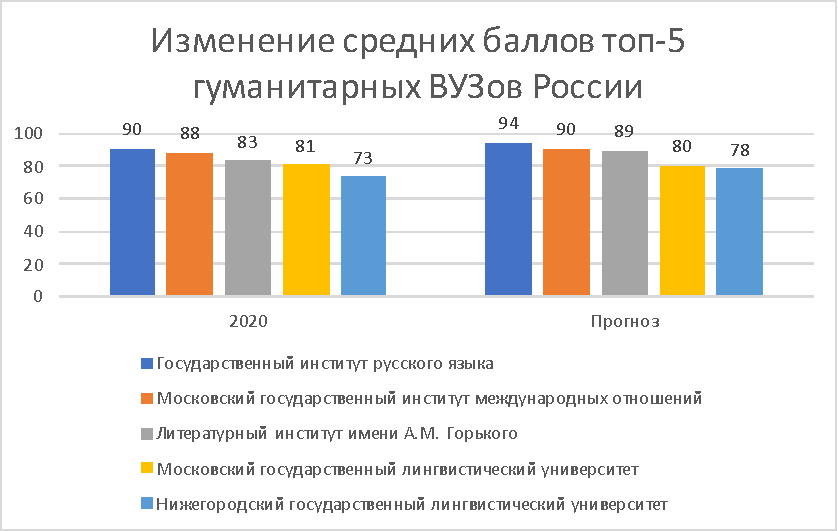
\includegraphics[scale=1.0]{img/top5gym.pdf.pdf}
	\caption{Изменение средних баллов ТОП-5 гуманитарных ВУЗов}
	\label{top5gym}
\end{figure} 	

На представленных результатах видно боковую динамику, резких изменений среднего балла не наблюдается.

\subsection{Различное количество бюджетных мест в ВУЗе}

Уменьшение количества бюджетных мест на 10\% во всех ВУЗах привело к повышение среднего балла, что видно на схемах, представленных ниже.

\begin{figure}[hbtp]
	\centering
	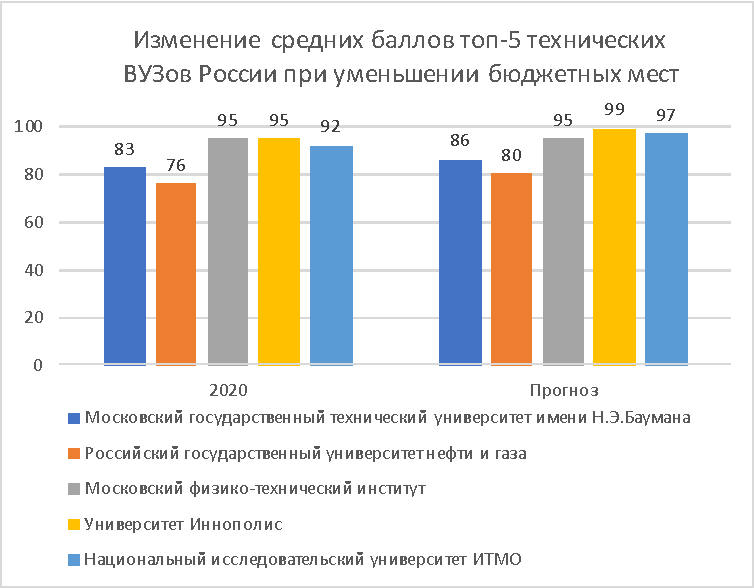
\includegraphics[scale=1.0]{img/top5techdown.pdf.pdf}
	\caption{Изменение средних баллов ТОП-5 технических ВУЗов при уменьшении бюджетных мест}
	\label{top5techdown}
\end{figure} 

\begin{figure}[hbtp]
	\centering
	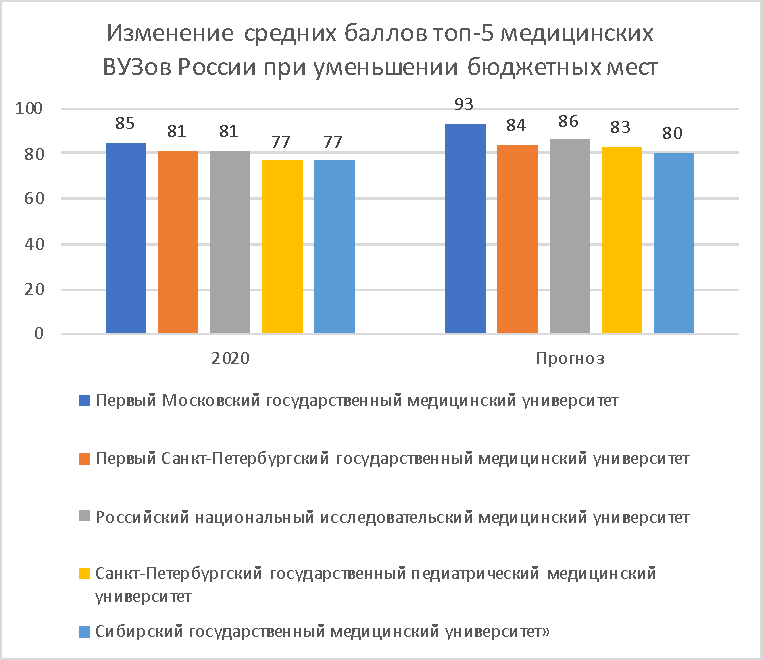
\includegraphics[scale=1.0]{img/top5meddown.pdf.pdf}
	\caption{Изменение средних баллов ТОП-5 медицинских ВУЗов при уменьшении бюджетных мест}
	\label{top5meddown}
\end{figure} 

\begin{figure}[hbtp]
	\centering
	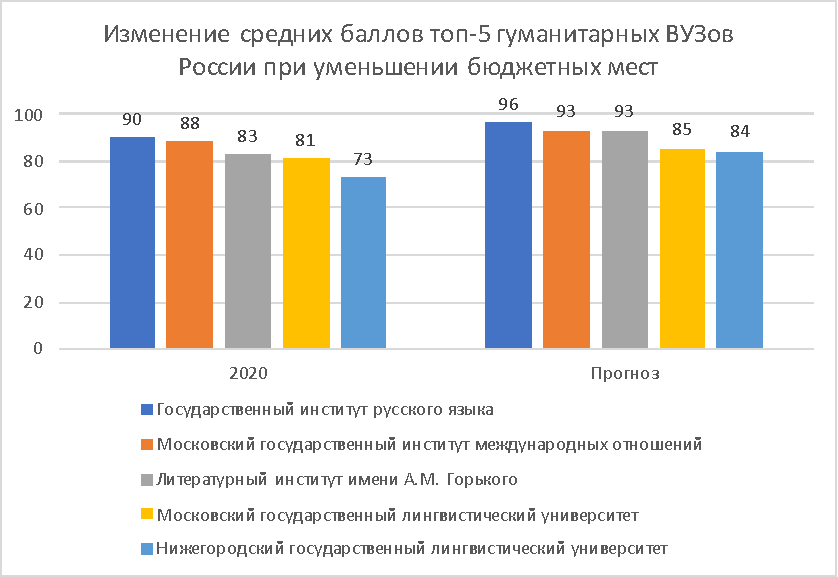
\includegraphics[scale=1.0]{img/top5gymdown.pdf.pdf}
	\caption{Изменение средних баллов ТОП-5 гуманитарных ВУЗов при уменьшении бюджетных мест}
	\label{top5gymdown}
\end{figure} 	

При увеличении количества бюджетных мест на 10\%, проходной балл уменьшился.

\begin{figure}[hbtp]
	\centering
	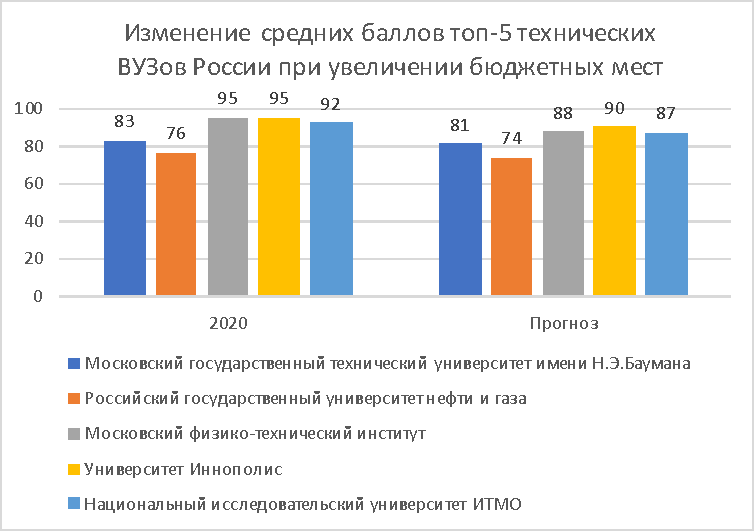
\includegraphics[scale=1.0]{img/top5techup.pdf.pdf}
	\caption{Изменение средних баллов ТОП-5 технических ВУЗов при увеличении бюджетных мест}
	\label{top5techup}
\end{figure} 

\begin{figure}[hbtp]
	\centering
	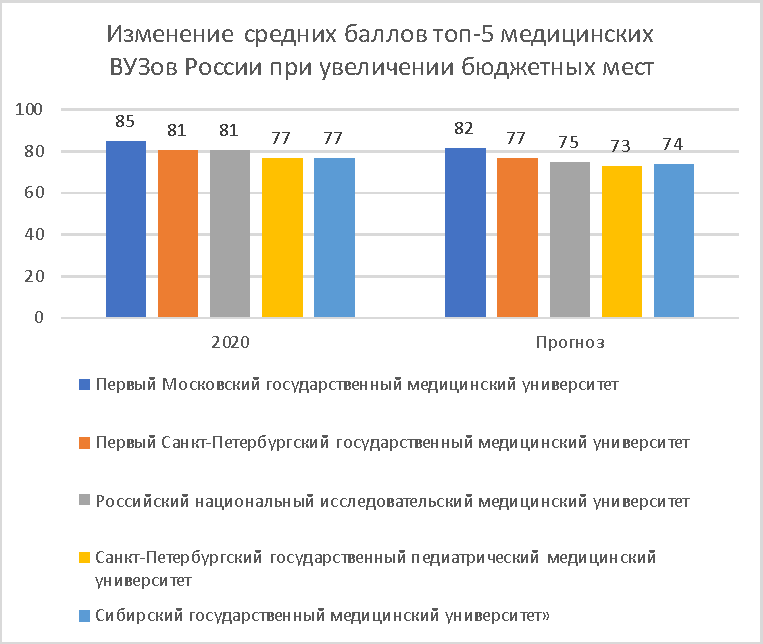
\includegraphics[scale=1.0]{img/top5medup.pdf.pdf}
	\caption{Изменение средних баллов ТОП-5 медицинских ВУЗов при увеличении бюджетных мест}
	\label{top5medup}
\end{figure} 

\begin{figure}[hbtp]
	\centering
	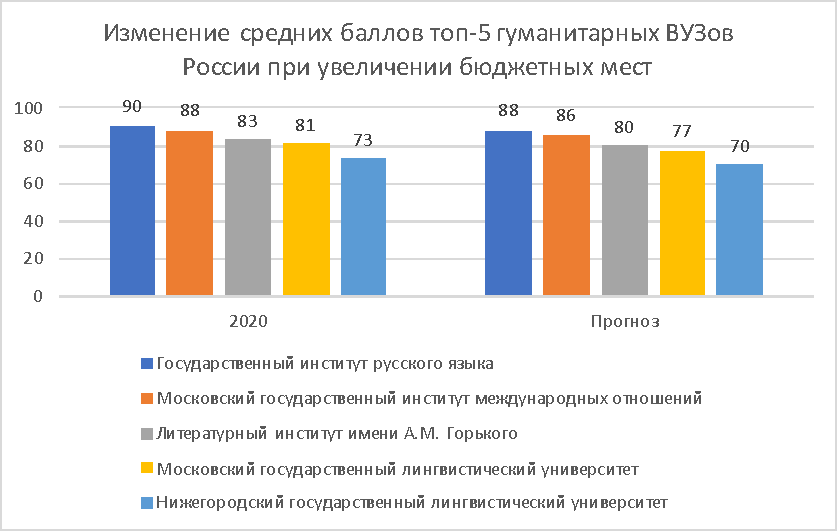
\includegraphics[scale=1.0]{img/top5gymup.pdf.pdf}
	\caption{Изменение средних баллов ТОП-5 гуманитарных ВУЗов при увеличении бюджетных мест}
	\label{top5gymup}
\end{figure} 	

\subsection{Увеличение максимального числа ВУЗов для подачи заявлений}

Для проведения исследования был запущен процесс моделирования с указанным в конфигурации максимальным числом 10 – количество ВУЗов для подачи заявлений.

\begin{figure}[hbtp]
	\centering
	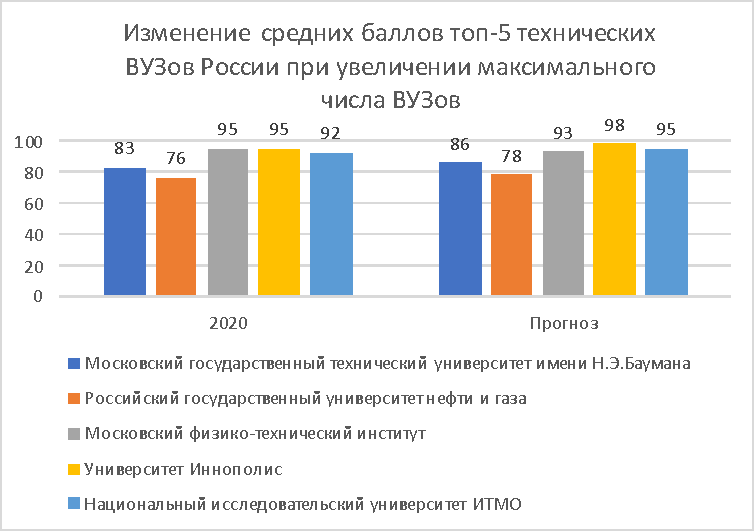
\includegraphics[scale=1.0]{img/top5techmax.pdf.pdf}
	\caption{Изменение средних баллов ТОП-5 технических ВУЗов при увеличении максимального числа ВУЗов}
	\label{top5techmax}
\end{figure} 

\begin{figure}[hbtp]
	\centering
	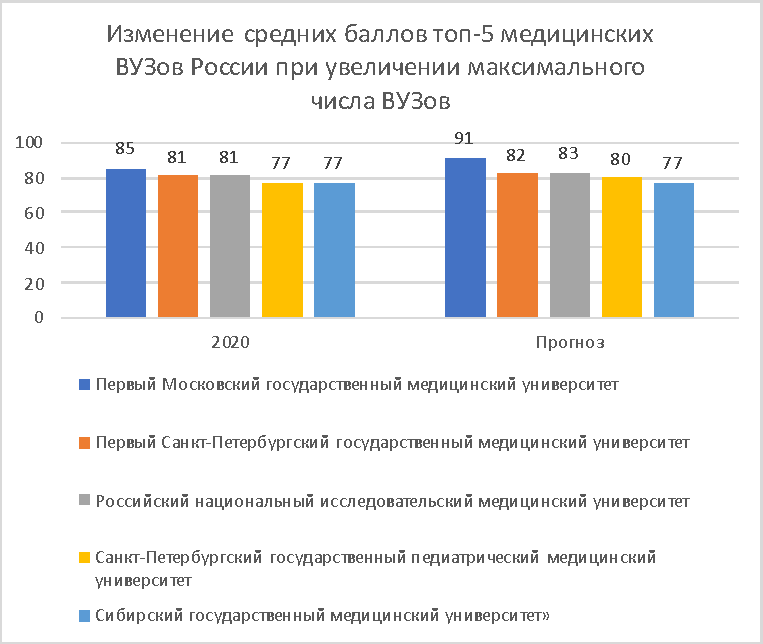
\includegraphics[scale=1.0]{img/top5medmax.pdf.pdf}
	\caption{Изменение средних баллов ТОП-5 медицинских ВУЗов при увеличении максимального числа ВУЗов}
	\label{top5medmax}
\end{figure} 

\begin{figure}[hbtp]
	\centering
	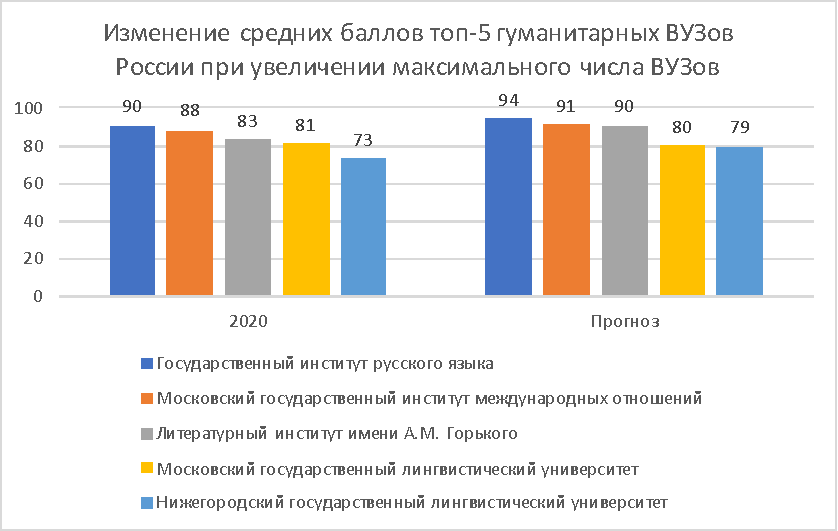
\includegraphics[scale=1.0]{img/top5gymmax.pdf.pdf}
	\caption{Изменение средних баллов ТОП-5 гуманитарных ВУЗов при увеличении максимального числа ВУЗов}
	\label{top5gymmax}
\end{figure} 	

В полученных результатах не наблюдаются значимые изменения среднего балла, что говорит о том, что абитуриенты в основном подают документы в заранее выбранное небольшое количество ВУЗов.

\subsection{Различные диапазоны результатов сдачи ЕГЭ}

Исследования выше проводились на основе трех заданных категорий агентов с соответствующими диапазонами баллов результатов ЕГЭ. Для исследования зависимости среднего балла от результатов ЕГЭ были изменены диапазоны в сторону увеличения на следующие:

\begin{itemize}[leftmargin=1.6\parindent]
	\item[---] 70-80 для первой категории;
	\item[---] 81-90 для второй категории;
	\item[---] 91-100 для третьей категории.
\end{itemize}

В результате получены следующие результаты при моделировании:

\begin{figure}[hbtp]
	\centering
	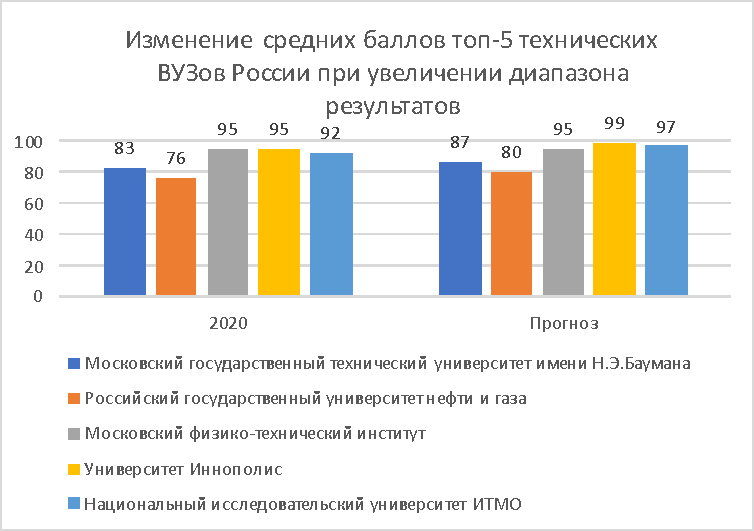
\includegraphics[scale=1.0]{img/top5techdur.pdf.pdf}
	\caption{Изменение средних баллов ТОП-5 технических ВУЗов при увеличении диапазона результатов}
	\label{top5techdur}
\end{figure} 

\begin{figure}[hbtp]
	\centering
	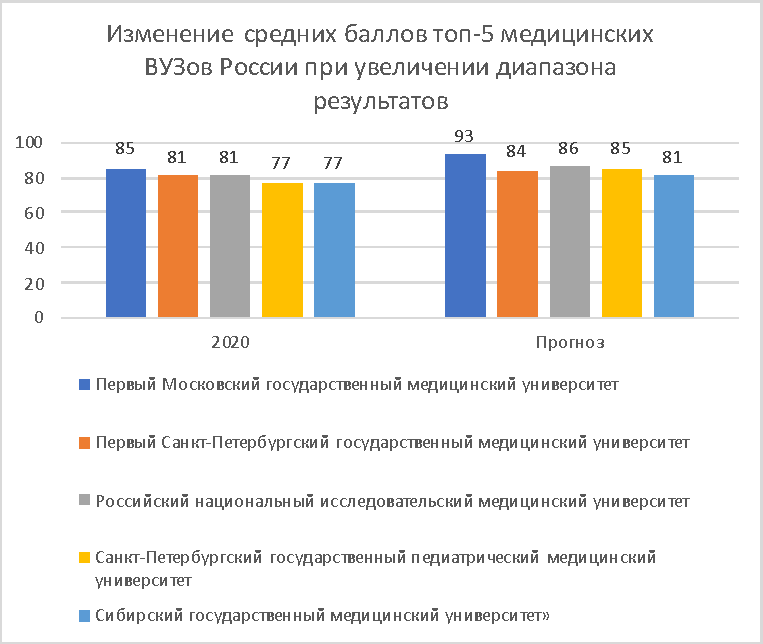
\includegraphics[scale=1.0]{img/top5meddur.pdf.pdf}
	\caption{Изменение средних баллов ТОП-5 медицинских ВУЗов при увеличении диапазона результатов}
	\label{top5meddur}
\end{figure} 

\begin{figure}[hbtp]
	\centering
	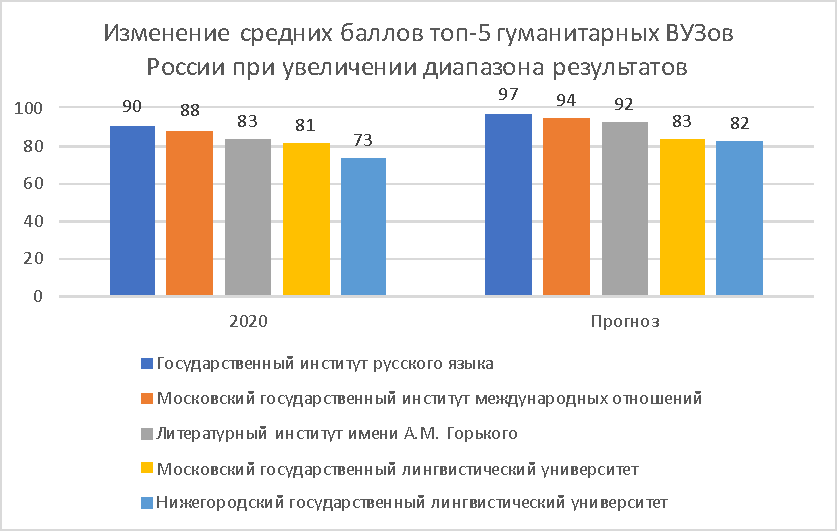
\includegraphics[scale=1.0]{img/top5gymdur.pdf.pdf}
	\caption{Изменение средних баллов ТОП-5 гуманитарных ВУЗов при увеличении диапазона результатов}
	\label{top5gymdur}
\end{figure} 	

В среднем увеличение среднего балла у каждого ВУЗа составило 5 баллов.

\pagebreak